\documentclass[11pt]{exam}
\usepackage[margin=1in]{geometry}
\usepackage{amsfonts, amsmath, amssymb, amsthm}
\usepackage{mathtools}
\usepackage{enumerate}
\usepackage{listings}
\usepackage{colortbl}
\usepackage{float}
\usepackage[colorlinks,linkcolor=blue]{hyperref}

% in order to compile this file you need to get 'header.tex' from
% Canvas and change the line below to the appropriate file path
%%% theorems

\theoremstyle{plain}            % following are "theorem" style
\newtheorem{theorem}{Theorem}[section]
\newtheorem{lemma}[theorem]{Lemma}
\newtheorem{corollary}[theorem]{Corollary}
\newtheorem{proposition}[theorem]{Proposition}
\newtheorem{claim}[theorem]{Claim}
\newtheorem{fact}[theorem]{Fact}
\newtheorem{openproblem}[theorem]{Open Problem}

\theoremstyle{definition}       % following are def style
\newtheorem{definition}[theorem]{Definition}
\newtheorem{conjecture}[theorem]{Conjecture}
\newtheorem{example}[theorem]{Example}
\newtheorem{protocol}[theorem]{Protocol}
\newtheorem{exercise}[theorem]{Exercise}

\theoremstyle{remark}           % following are remark style
\newtheorem{remark}[theorem]{Remark}
\newtheorem{note}[theorem]{Note}
%\newtheorem*{solution}{Solution}

%%% special sets
\newcommand{\bit}{\ensuremath{\{0,1\}}}
\newcommand{\bitt}{\ensuremath{\{-1,1\}}}
\newcommand{\ball}{\ensuremath{\mathcal{B}}}
\newcommand{\sph}{\ensuremath{\mathbb{S}}}
\newcommand{\odisc}[2]{\ensuremath{D(#1, #2)}}
\newcommand{\cdisc}[2]{\ensuremath{\bar{D}(#1, #2)}}
\newcommand{\emp}{\varnothing}

% constants
\newcommand{\E}{\ensuremath{\mathrm{e}}}
\newcommand{\I}{\ensuremath{\mathrm{i}}}
\newcommand{\Id}{\ensuremath{\mathrm{I}}}
\newcommand{\paulix}{\ensuremath{\mathrm{X}}}
\newcommand{\pauliy}{\ensuremath{\mathrm{Y}}}
\newcommand{\pauliz}{\ensuremath{\mathrm{Z}}}

% font for general-purpose algorithms
\newcommand{\algo}[1]{\ensuremath{\mathsf{#1}}}
% font for general-purpose computational problems
\newcommand{\problem}[1]{\ensuremath{\mathsf{#1}}}
% font for complexity classes
\newcommand{\class}[1]{\ensuremath{\mathsf{#1}}}

% asymptotics
\DeclareMathOperator{\poly}{poly}
\DeclareMathOperator{\polylog}{polylog}
\DeclareMathOperator{\negl}{negl}
\DeclareMathOperator{\bigO}{O}
\DeclareMathOperator{\litO}{o}
\DeclareMathOperator{\Otil}{\tilde{O}}
\DeclareMathOperator{\Ostar}{O^*}

%%% "LEFT-RIGHT" PAIRS OF SYMBOLS

% inner product
\DeclarePairedDelimiter\inner{\langle}{\rangle}
% absolute value
\DeclarePairedDelimiter\abs{\lvert}{\rvert}
% a set
\DeclarePairedDelimiter\set{\{}{\}}
% parens
\DeclarePairedDelimiter\parens{(}{)}
% tuple, alias for parens
\DeclarePairedDelimiter\tuple{(}{)}
% square brackets
\DeclarePairedDelimiter\bracks{[}{]}
% rounding off
\DeclarePairedDelimiter\round{\lfloor}{\rceil}
% floor function
\DeclarePairedDelimiter\floor{\lfloor}{\rfloor}
% ceiling function
\DeclarePairedDelimiter\ceil{\lceil}{\rceil}
% length of some vector, element
\DeclarePairedDelimiter\length{\lVert}{\rVert}
% "lifting" of a residue class
\DeclarePairedDelimiter\lift{\llbracket}{\rrbracket}
\DeclarePairedDelimiter\len{\lvert}{\rvert}
% bra-kets
\DeclarePairedDelimiter\bra{\langle}{\rvert}
\DeclarePairedDelimiter\ket{\lvert}{\rangle}
\newcommand{\braket}[2]{\ensuremath{\langle #1 \vert #2 \rangle}}
\newcommand{\ketbra}[2]{\ensuremath{\lvert #1 \rangle \langle #2 \rvert}}

%%% spacing

\newcommand{\ws}{\hspace{1pt}}
\newcommand{\wws}{\hspace{2pt}}
\newcommand{\hs}{\hspace{4pt}}
\newcommand{\hhs}{\hspace{8pt}}
\newcommand{\hhhs}{\hspace{12pt}}

%%% LISTS

\newcommand{\oneto}{1, \ldots,}
\newcommand{\onetop}{1 \cdots,}
\newcommand{\zeroto}{0, \ldots,}
\newcommand{\zerotop}{0 \cdots,}
\newcommand{\perm}[1]{\mathbf{(#1)}}
\newcommand{\permv}[1]{(#1)}
\newcommand{\varind}[2]{#1_1, \ldots, #1_#2}
\newcommand{\varindz}[2]{#1_0, \ldots, #1_#2}
\newcommand{\varindp}[2]{#1_1 \cdots #1_#2}
\newcommand{\varindpz}[2]{#1_0 \cdots #1_#2}
\newcommand{\seq}[2]{(#1_#2)_{#2=1}^\infty}
\newcommand{\seqz}[2]{(#1_#2)_{#2=0}^\infty}

%%% MATH OPERATORS

%\DeclareMathOperator{\pr}{\mathbf{P}}
%\DeclareMathOperator{\ex}{\mathbf{E}}
\DeclareMathOperator{\pr}{P}
\DeclareMathOperator{\ex}{E}
\DeclareMathOperator{\Span}{Span}
\DeclareMathOperator{\tr}{Tr}
\DeclareMathOperator{\supp}{Supp}
\DeclareMathOperator{\im}{Im}
\DeclareMathOperator{\var}{var}
\DeclareMathOperator{\vol}{vol}
\DeclareMathOperator{\sign}{sign}
\DeclareMathOperator{\dkl}{D_{KL}}
\DeclareMathOperator{\entr}{H}
\DeclareMathOperator{\fid}{F}
\DeclareMathOperator{\dist}{D}
\DeclareMathOperator{\ad}{ad}

% hats

\newcommand{\fhat}{\ensuremath{\hat{f}}}
\newcommand{\phat}{\ensuremath{\hat{p}}}
\newcommand{\that}{\ensuremath{\hat{t}}}

%%% BLACKBOARD SYMBOLS

% \newcommand{\C}{\ensuremath{\mathbb{C}}}
\newcommand{\D}{\ensuremath{\mathbb{D}}}
\newcommand{\F}{\ensuremath{\mathbb{F}}}
% \newcommand{\G}{\ensuremath{\mathbb{G}}}
\newcommand{\J}{\ensuremath{\mathbb{J}}}
\newcommand{\N}{\ensuremath{\mathbb{N}}}
\newcommand{\Q}{\ensuremath{\mathbb{Q}}}
\newcommand{\R}{\ensuremath{\mathbb{R}}}
\newcommand{\T}{\ensuremath{\mathbb{T}}}
\newcommand{\Z}{\ensuremath{\mathbb{Z}}}
\newcommand{\QR}{\ensuremath{\mathbb{QR}}}

% sets in calligraphic type

\newcommand{\calD}{\ensuremath{\mathcal{D}}}
\newcommand{\calF}{\ensuremath{\mathcal{F}}}
\newcommand{\calG}{\ensuremath{\mathcal{G}}}
\newcommand{\calH}{\ensuremath{\mathcal{H}}}
\newcommand{\calI}{\ensuremath{\mathcal{I}}}
\newcommand{\calL}{\ensuremath{\mathcal{L}}}
\newcommand{\calN}{\ensuremath{\mathcal{N}}}
\newcommand{\calP}{\ensuremath{\mathcal{P}}}
\newcommand{\calS}{\ensuremath{\mathcal{S}}}
\newcommand{\calX}{\ensuremath{\mathcal{X}}}
\newcommand{\calY}{\ensuremath{\mathcal{Y}}}

% matrices and vectors

\newcommand{\matA}{\ensuremath{\mathbf{A}}}
\newcommand{\matB}{\ensuremath{\mathbf{B}}}
\newcommand{\matC}{\ensuremath{\mathbf{C}}}
\newcommand{\matD}{\ensuremath{\mathbf{D}}}
\newcommand{\matE}{\ensuremath{\mathbf{E}}}
\newcommand{\matF}{\ensuremath{\mathbf{F}}}
\newcommand{\matG}{\ensuremath{\mathbf{G}}}
\newcommand{\matH}{\ensuremath{\mathbf{H}}}
\newcommand{\matI}{\ensuremath{\mathbf{I}}}
\newcommand{\matJ}{\ensuremath{\mathbf{J}}}
\newcommand{\matK}{\ensuremath{\mathbf{K}}}
\newcommand{\matL}{\ensuremath{\mathbf{L}}}
\newcommand{\matM}{\ensuremath{\mathbf{M}}}
\newcommand{\matN}{\ensuremath{\mathbf{N}}}
\newcommand{\matO}{\ensuremath{\mathbf{O}}}
\newcommand{\matP}{\ensuremath{\mathbf{P}}}
\newcommand{\matQ}{\ensuremath{\mathbf{Q}}}
\newcommand{\matR}{\ensuremath{\mathbf{R}}}
\newcommand{\matS}{\ensuremath{\mathbf{S}}}
\newcommand{\matT}{\ensuremath{\mathbf{T}}}
\newcommand{\matU}{\ensuremath{\mathbf{U}}}
\newcommand{\matV}{\ensuremath{\mathbf{V}}}
\newcommand{\matW}{\ensuremath{\mathbf{W}}}
\newcommand{\matX}{\ensuremath{\mathbf{X}}}
\newcommand{\matY}{\ensuremath{\mathbf{Y}}}
\newcommand{\matZ}{\ensuremath{\mathbf{Z}}}
\newcommand{\matzero}{\ensuremath{\mathbf{0}}}

\newcommand{\veca}{\ensuremath{\mathbf{a}}}
\newcommand{\vecb}{\ensuremath{\mathbf{b}}}
\newcommand{\vecc}{\ensuremath{\mathbf{c}}}
\newcommand{\vecd}{\ensuremath{\mathbf{d}}}
\newcommand{\vece}{\ensuremath{\mathbf{e}}}
\newcommand{\vecf}{\ensuremath{\mathbf{f}}}
\newcommand{\vecg}{\ensuremath{\mathbf{g}}}
\newcommand{\vech}{\ensuremath{\mathbf{h}}}
\newcommand{\veck}{\ensuremath{\mathbf{k}}}
\newcommand{\vecm}{\ensuremath{\mathbf{m}}}
\newcommand{\vecp}{\ensuremath{\mathbf{p}}}
\newcommand{\vecq}{\ensuremath{\mathbf{q}}}
\newcommand{\vecr}{\ensuremath{\mathbf{r}}}
\newcommand{\vecs}{\ensuremath{\mathbf{s}}}
\newcommand{\vect}{\ensuremath{\mathbf{t}}}
\newcommand{\vecu}{\ensuremath{\mathbf{u}}}
\newcommand{\vecv}{\ensuremath{\mathbf{v}}}
\newcommand{\vecw}{\ensuremath{\mathbf{w}}}
\newcommand{\vecx}{\ensuremath{\mathbf{x}}}
\newcommand{\vecy}{\ensuremath{\mathbf{y}}}
\newcommand{\vecz}{\ensuremath{\mathbf{z}}}
\newcommand{\veczero}{\ensuremath{\mathbf{0}}}
\newcommand{\vecone}{\ensuremath{\mathbf{1}}}

\newcommand{\vecell}{\ensuremath{\boldsymbol\ell}}
\newcommand{\vecalpha}{\ensuremath{\boldsymbol\alpha}}
\newcommand{\vecbeta}{\ensuremath{\boldsymbol\beta}}
\newcommand{\veceta}{\ensuremath{\boldsymbol\eta}}
\newcommand{\vecmu}{\ensuremath{\boldsymbol\mu}}
\newcommand{\vecphi}{\ensuremath{\boldsymbol\phi}}
\newcommand{\vecsigma}{\ensuremath{\boldsymbol\sigma}}
\newcommand{\vectheta}{\ensuremath{\boldsymbol\theta}}
\newcommand{\vecxi}{\ensuremath{\boldsymbol\xi}}

%%% misc

\newcommand{\ind}{\ensuremath{\mathbf{1}}}

\newcommand{\congmod}[3]{#1 \equiv #2 \textrm{ modulo } #3}

\newcommand{\dee}{\,\mathrm{d}}
\newcommand{\de}{\mathrm{d}}
\newcommand{\dx}{\,\mathrm{d} x}

\newcommand{\ol}{\overline}
\newcommand{\inv}[1]{\ensuremath{#1^{-1}}}
\newcommand{\tsp}[1]{\ensuremath{#1^{\top}}}


\newcommand{\eps}{\varepsilon}
\newcommand{\ph}{\varphi}

\newcommand{\Ra}{\Rightarrow}
\newcommand{\Lra}{\Leftrightarrow}
\newcommand{\rsqa}{\rightsquigarrow}

\newcommand{\trl}{\triangleleft}
\newcommand{\trr}{\triangleright}

\newcommand{\func}[3]{#1: #2 \to #3}
\newcommand{\dd}[1]{\frac{\mathrm{d}}{\mathrm{d}#1}}
\newcommand{\ptl}[1]{\frac{\partial}{\partial #1}}
\newcommand{\prtl}[2]{\frac{\partial #1}{\partial #2}}

\newcommand{\matrixtt}[4]{
  \begin{pmatrix*}[r]
        #1 & #2 \\
        #3 & #4
    \end{pmatrix*}
}

%%% for homework and section notes

\newcommand{\commonheader}[2]{
    \pagestyle{headandfoot}
    \setlength{\headheight}{26pt}
    \setlength{\headsep}{30pt}

    \header
        {\small{\textbf{VE281: Data Structures and Algorithms}} \\ \footnotesize{\textbf{UM-SJTU Joint Institute, FA2022}}}
        {#1}
        {#2}

    \firstpageheadrule
    \runningheadrule

    \footer
        {}
        {\thepage}
        {}
}

\newcommand{\hwheader}{
    \commonheader
        {\textbf{Homework \hwnum}}
        {\small \textbf{Due at \duedate}}
}

\newcommand{\hwslnheader}{
    \commonheader
    	{}
        {\textbf{Solutions to Homework \hwnum}}
    \printanswers
}

\newcommand{\notesheader}{
    \commonheader
        {\Large \textbf{Section Notes \sectionnum}}
    	{}
}

\newcommand{\hint}[1]{
\emph{Hint}: #1
}

% for effort questions
\let\Eitem=\relax
\def\effortE{\textbf{E}~}
\makeatletter
\def\Eitem{%
    \expandafter\let\expandafter\originallabel\csname labelenum\romannumeral\@enumdepth\endcsname
    \expandafter\def\csname labelenum\romannumeral\@enumdepth\expandafter\endcsname\expandafter{%
        \expandafter\effortE\originallabel}%
    \item
    \expandafter\let\csname labelenum\romannumeral\@enumdepth\endcsname\originallabel
}
\makeatother

\allowdisplaybreaks


\geometry{left=2.5 cm,right=2.5 cm,top=2.5 cm,bottom=2.5 cm}
%\pagestyle{fancy}
\definecolor{mygreen}{rgb}{0,0.6,0}  
\definecolor{mygray}{rgb}{0.5,0.5,0.5}
\definecolor{mymauve}{rgb}{0.58,0,0.82} 
\definecolor{background}{rgb}{0.963,0.963,0.963}

\definecolor{codegreen}{rgb}{0,0.6,0}
\definecolor{codegray}{rgb}{0.5,0.5,0.5}
\definecolor{codepurple}{rgb}{0.58,0,0.82}
\definecolor{backcolour}{rgb}{0.95,0.95,0.92}

\lstdefinestyle{mystyle}{
    backgroundcolor=\color{backcolour},   
    commentstyle=\color{codegreen},
    keywordstyle=\color{magenta},
    numberstyle=\tiny\color{codegray},
    stringstyle=\color{codepurple},
    basicstyle=\ttfamily\footnotesize,
    breakatwhitespace=false,         
    breaklines=true,                 
    captionpos=b,                    
    keepspaces=true,                 
    numbers=left,                    
    numbersep=5pt,                  
    showspaces=false,                
    showstringspaces=false,
    showtabs=false,                  
    tabsize=2
}

\lstset{style=mystyle}
\newcommand{\hwnum}{2}
\newcommand{\duedate}{2022.11.14}

%\notesheader
\hwheader   % header for homework
%\hwslnheader   % header for homework solutions

% Comment the following line in order to hide solutions.
% Uncomment the line to show solutions written inside of
% LaTeX solution environments like:
%   \begin{solution}
%     My solution.
%   \end{solution}.
\printanswers

\begin{document}
\setlength{\parindent}{0pt}
\section*{Before you start:}

\subsection*{Homework Files}
You can download the starter files for coding as well as this \textit{tex} file (you only need to modify \textit{homework2.tex}) on canvas and do your homework with latex. Or you can scan your handwriting, convert to pdf file, and upload it to canvas before the due date. If you choose to write down your answers by hand, you can directly download the pdf file on canvas which provides more blank space for solution box.\\

\subsection*{Submission Form}
A pdf file as your solution named as VE281\_HW2\_[Your Student ID]\_[Your name].pdf uploaded to canvas


Estimated time used for this homework: \textbf{3-4 hours.}
\\\\


\newpage
\section*{0\quad Student Info}
Your name and student id:
\begin{solution}
    % Write your answer here
\end{solution}
\section{Choices (16 points)}
\begin{enumerate}
    \item For hashing the array (7,34,55,25,64,46,20,10), if H (K)=K\%9 is used as the hash function,
          how many pairs of elements are hashed with address 1?
          \begin{enumerate}[A.]
              \item 1
              \item 2
              \item 3
              \item 4
          \end{enumerate}
          \begin{solution}
              % Write your answer here
          \end{solution}
    \item Let the length of the hash table be 14, the hash function be H(key)=key\%11, and the existing data in the table have four key words: 15,38,61,84. Now, the element with key word 49 is added to the table, and the conflict is resolved by two probing methods.
          Which position is the place to put in?
          \begin{enumerate}
              \item 8
              \item 3
              \item 5
              \item 9
          \end{enumerate}
          \begin{solution}
              % Write your answer here
          \end{solution}
    \item Which of the following statements about hash lookup is not true?
          \begin{enumerate}
              \item With the chain-address approach, it takes the same amount of time to find an element
              \item When using the chain address method to handle conflicts, if the insertion rule is always at the beginning of the chain, the time to insert either element is the same
              \item Using the chain address method to deal with the conflict will not cause the secondary aggregation phenomenon
              \item The chain address method is used to deal with conflicts, which is suitable for uncertain table length

          \end{enumerate}
          \begin{solution}
              % Write your answer here
          \end{solution}
    \item Have a set of data (15,9,7,8,20, 1,7,4), established by screening method descending sort heap sort of initial heap for ()
          \begin{enumerate}
              \item  -1,4,8,9,20,7,15,7
              \item  -1,7,15,7,4,8,20,9
              \item  -1,4,15,9,20,7,7,8
              \item  -1,4,7,8,20,15,7,9
          \end{enumerate}
          \begin{solution}
              % Write your answer here
          \end{solution}
\end{enumerate}
\section{Tree and Heap (34 points) }
\subsection{Leaf (2+3+3+3 points)}
\begin{enumerate}
    \item
          A proper binary tree has $n$ 2-degree nodes, what is the number of leaf nodes?
          \begin{solution}
              % Write your answer here
          \end{solution}
    \item
          Try to prove that for a heap with n nodes, the index of the leaves goes from $floor(n/2)+1$ to $n$
          \begin{solution}
              % write your solution here
          \end{solution}
    \item
          Try to prove that for a heap with n nodes, there are at most $ceiling(\frac{n}{2^{(h+1)}})$ nodes with height h.
          \begin{solution}
              % write your solution here
          \end{solution}
    \item  What's the number of leaf nodes for a complete binary tree with $n$ nodes? (Elaborate your solution)
          \begin{solution}
              % Write your answer here
          \end{solution}

\end{enumerate}
\subsection{Traversal (5 points)}
Given the pre-order traversal $\{1,3,2,10,6,5,4,8,11,9,22,12\}$\\
and in-order traversal
$\{10,2,6,3,5,1,11,8,4,22,9,12\}$, draw the tree and write down the post-order
and level-order traversal (null node marked).
\begin{solution}
    % Write your answer here
\end{solution}
\subsection{Initial(8 points)}
If we want to initialize a minHeap with n elements. Recall that the min heap initialization
algorithm can reduce the time complexity from $O(n\log n)$ to $O(n)$. Now lets us apply this
algorithm to insert the following integers.
100, 76, 50, 12, 21, 42, 44, 93, 91, 51, 26, 29, 99, 88, 64, 70, 78, 19, 31.
What is the total number of function call percolateDown and the number of swaps operation
in it?
\begin{solution}
    % Write your answer here
\end{solution}
\subsection{Structure (10 points)}
What is the number of possible proper binary tree structures giving the fact that it has 13 nodes?
(Elaborate your solution. This question is \textbf{difficult}!)
\begin{solution}
    % Write your answer here
\end{solution}


\section{Hashing Zoo (20 points)}
Suppose Prof. Blue Tiger is using a hash table to store information about the grades of his students. The keys are strings and the values are integers. Furthermore, he uses a very simple function t where the hash code of a string is its length. For example:
\begin{itemize}
    \item t("Blue Tiger") = 10
    \item t("Red Flamingo") = 12
    \item t("Glass Frog") = 10
\end{itemize}
One of his TA gives another function t where the hash code of a string is the integer representing its last letter.
For example:
\begin{itemize}
    \item t("Blue Tiger") = 17
    \item t("Red Flamingo") = 14
    \item t("Glass Frog") = 6
\end{itemize}
And we have:
\begin{table}[H]
    \centering
    \setlength{\tabcolsep}{1mm}
    \begin{tabular}{cccccccccccccccccccccccccc}
        a & b & c & d & e & f & g & h & i & j & k  & l  & m  & n  & o  & p  & q  & r  & s  & t  & u  & v  & w  & x  & y  & z  \\
        0 & 1 & 2 & 3 & 4 & 5 & 6 & 7 & 8 & 9 & 10 & 11 & 12 & 13 & 14 & 15 & 16 & 17 & 18 & 19 & 20 & 21 & 22 & 23 & 24 & 25
    \end{tabular}
\end{table}

\subsection{Hash Function (3 points)}
Which function would be better? State your reason.

\begin{solution}
    % write your answer here
\end{solution}

Prof. Blue Tiger decides to use the second function and work with a hash table of size 13. The hash function is $h(t) = t \;\%\; 13$. This means that "Red Flamingo" would hash to 14, but ultimately fall into bucket $14 \;\%\; 13 = 1$ of our table. For this problem, you will determine where each of the given name lands after inserting a sequence of values using three different collision resolution schemes:

\begin{itemize}
    \item linear probing
    \item quadratic probing
    \item double hashing with $h_i(t) = h(h(t)+((13-t)\;\%\; 10) * i)$
\end{itemize}

For each of these three collision resolution schemes, determine the resulting hash table after inserting the following $(key,\;value)$ pairs in the given order:
\begin{enumerate}[1.]
    \item ("Blue Tiger", 100)
    \item ("Red Flamingo", 88)
    \item ("Rainbow Horse", 80)
    \item ("Honeydew Alligator", 70)
    \item ("Pink Elephant", 101)
    \item ("Gold Monkey", 65)
    \item ("Glass Fish", 96)
    \item ("Yellow Dog", 87)
\end{enumerate}

\textbf{Every incorrect value counts for 0.5 point.}
\subsection{Linear Probing (4 points)}
Please use the \textbf{linear probing} collision resolution method to simulate the given insertion steps, and then show the final position of each $value$ inside the related buckets below.
\begin{solution}
    \begin{table}[H]
        \centering
        \renewcommand{\arraystretch}{2}
        \resizebox{\linewidth}{!}{
            \begin{tabular}{|c|c|c|c|c|c|c|c|c|c|c|c|c|c|c|c|c|}
                \hline
                \textbf{Index} & 0 & 1 & 2 & 3 & 4 & 5 & 6 & 7 & 8 & 9 & 10 & 11 & 12 \\
                \hline
                \textbf{Value} &   &   &   &   &   &   &   &   &   &   &    &    &    \\
                \hline
            \end{tabular}}
    \end{table}
\end{solution}
\subsection{Quadratic Probing (4 points)}
Please use the \textbf{quadratic probing} collision resolution method to simulate the given insertion steps, and then show the final position of each $value$ pair inside the related buckets below.
\begin{solution}
    \begin{table}[H]
        \centering
        \renewcommand{\arraystretch}{2}
        \resizebox{\linewidth}{!}{
            \begin{tabular}{|c|c|c|c|c|c|c|c|c|c|c|c|c|c|c|c|c|}
                \hline
                \textbf{Index} & 0 & 1 & 2 & 3 & 4 & 5 & 6 & 7 & 8 & 9 & 10 & 11 & 12 \\
                \hline
                \textbf{Value} &   &   &   &   &   &   &   &   &   &   &    &    &    \\
                \hline
            \end{tabular}}
    \end{table}
\end{solution}

\subsection{Double Hashing (4 points)}
Please use the \textbf{double hashing} collision resolution method to simulate the given insertion steps, with the double hash function $h_i(t) = h(h(t)+((13-t)\;\%\; 10) * i)$, and then show the final position of each $value$ pair inside the related buckets below.
\begin{solution}
    \begin{table}[H]
        \centering
        \renewcommand{\arraystretch}{2}
        \resizebox{\linewidth}{!}{
            \begin{tabular}{|c|c|c|c|c|c|c|c|c|c|c|c|c|c|c|c|c|}
                \hline
                \textbf{Index} & 0 & 1 & 2 & 3 & 4 & 5 & 6 & 7 & 8 & 9 & 10 & 11 & 12 \\
                \hline
                \textbf{Value} &   &   &   &   &   &   &   &   &   &   &    &    &    \\
                \hline
            \end{tabular}}
    \end{table}
\end{solution}

\subsection{Possible Insertion Order (5 points)}
Suppose you have a hash table of size 11 storing Blue Tiger's family members' favorite letter which shares the same t(key) and h(t). It uses open addressing with linear probing. After entering six values into the empty hash table, the state of the table is shown below.

\begin{table}[H]
    \centering
    \setlength{\tabcolsep}{5.5mm}
    \begin{tabular}{|c|c|c|c|c|c|c|c|c|c|c|c|}
        \hline
        \textbf{Index} & 0 & 1 & 2 & 3 & 4 & 5 & 6 & 7 & 8 & 9 & 10 \\
        \hline
        \textbf{Key}   & a & l & x & z & d & w &   &   &   &   &    \\
        \hline
    \end{tabular}
\end{table}
How many insertion orders are possible? Explain your answer clearly.

\begin{solution}
    % write your answer here
\end{solution}
\section{Binomial heap (30 points)}
A binomial heap is a data structure that acts as a priority queue but also allows pairs of heaps to be merged.
A binomial heap is implemented as a set of binomial trees (compare with a binary heap, which has a shape of a single binary tree), which are defined recursively as follows

1. binomial tree of order 0 is a single node.

2. binomial tree of order k ${\displaystyle k}$ k has a root node whose children are roots of binomial trees of orders $k - 1, k - 2 , ..., 2, 1, 0 $(in this order).

\begin{figure}[H]
    \begin{small}
        \begin{center}
            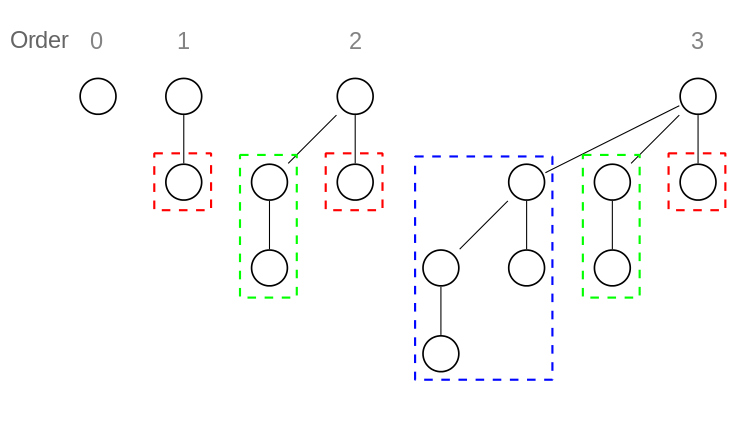
\includegraphics[width=0.5\textwidth]{./pic1.png}
        \end{center}
        \caption{Binomial heap}
    \end{small}
\end{figure}

A binomial heap is implemented as a set of binomial trees that satisfy the binomial heap properties:

1. Each binomial tree in a heap obeys the maximum-heap property: the key of a node is less than or equal to the key of its parent.

2. There can be at most one binomial tree for each order, including zero order.


\subsection{Merge (8 points)}

Here we provide a pseudo code to merge trees.
\begin{lstlisting}[]
Input : p,q as two trees
Output : a merged new tree 
function mergeTree(p, q)
    if p.root->key < q.root->key
        return q.addSubTree(p);
    else
        return p.addSubTree(q);   
\end{lstlisting}
Here we provide a pseudo code to check whether a tree is empty.
\begin{lstlisting}[]
Input : p as a tree
Output : whether p is empty
function isEmpty(p)
    if p.root==NULL 
        return true;
    else
        return false;
\end{lstlisting}

Please complete the pseudo code for merge two heaps. Each blank may have more than one statement.
\begin{lstlisting}[]
Input : p,q as two heaps (a list of trees sorted from order 0 to order k)
Output : heap as merged heap
function mergeHeap(p, q)
    heap=new Heap();
    pIt = p.head();
    qIt = q.head();
    heapIt = heap.head();
    while ([1])
        tree = mergeTree(*pIt,*qIt);
        if ([2])
            tree = mergeTree(tree, *heapIt);
        [3]
        pIt++;
        qIt++;
    return heap
\end{lstlisting}
\begin{solution}
    % Write your answer here
\end{solution}
\subsection{Delete (22 points)}
Please write a pseudo code to delete an element by its pointer. Hint: You can write $dequeMax$(10 points) and $increaseKey$(7 points) as helpers.
\begin{solution}
    % Write your answer here
\end{solution}
\section{RB tree}
\subsection{Path length}
Among the path from Node x to leaf node, is there one path that is greater than the double of that of another path? Prove your conclusion.
\begin{solution}
% Write your answer here
\end{solution}
\subsection{Init}
Init a tree by $insert$ function. How many nodes are needed to ensure that there is a red node in the tree?
\begin{solution}
% Write your answer here
\end{solution}
\subsection{Root node}
Why the root node must be black? What will happen is root node is red?
\begin{solution}
% Write your answer here
\end{solution}
\subsection{Insert}
Draw the tree after insert 2,4,3,0,5 into the tree. There is one node (Black 1) in the tree at first.
\begin{solution}
    % Write your answer here
\end{solution}
\end{document}